\section{Static-Network Analysis}

\subsection{Small World}
At the book's end, the largest component has 224 nodes and the diameter is 5.
Since $ln(224) = 5.41$, we see that this network does indeed display the small world property, similar to real-world social networks.

\subsection{Degree Distribution}

\begin{figure}[ht]
    \centering
    \begin{subfigure}{0.4\textwidth}
        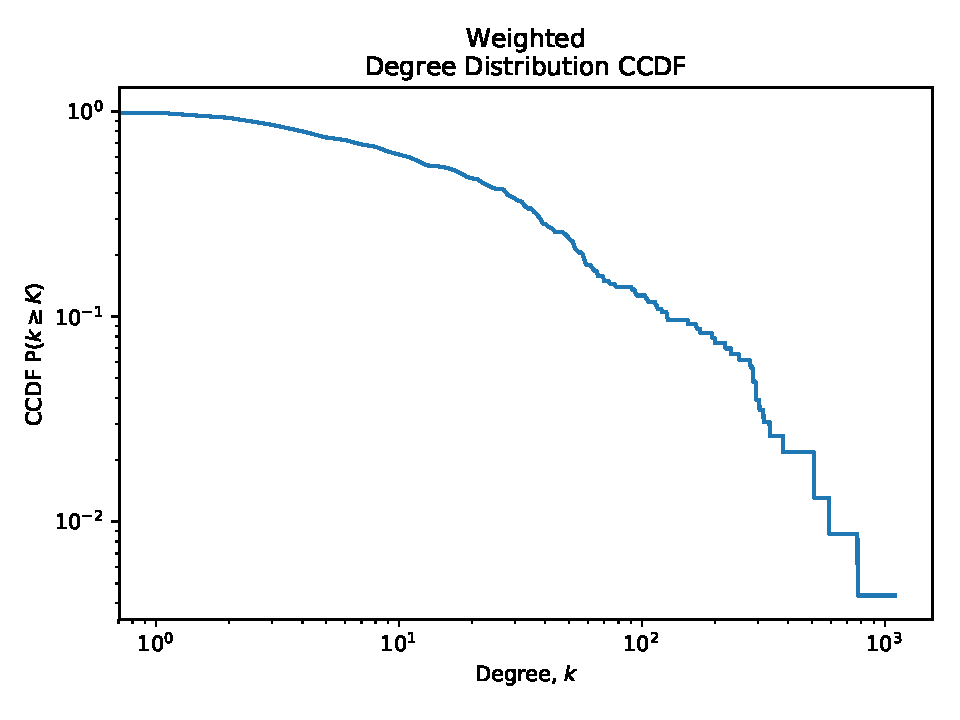
\includegraphics[width=1.\textwidth]{images/weighted_degree_distr_ccdf.pdf}
        \caption{Weighted degree distribution.}
    \end{subfigure}
    \begin{subfigure}{0.4\textwidth}
        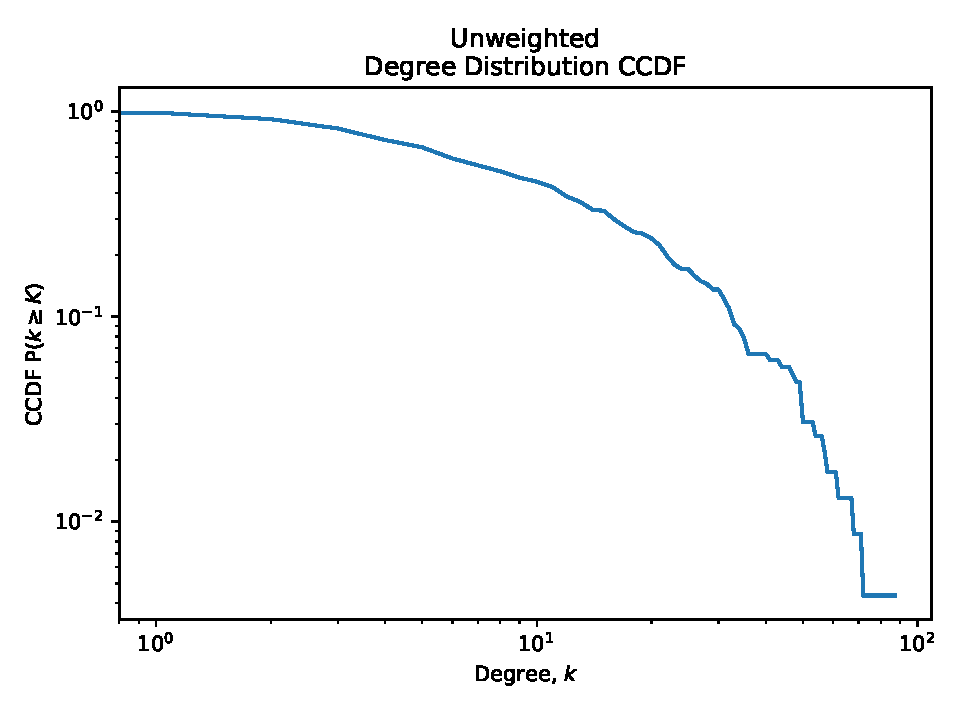
\includegraphics[width=1.\textwidth]{images/unweighted_degree_distr_ccdf.pdf}
        \caption{Unweighted degree distribution.}
    \end{subfigure}
    \caption{Degree distributions on a log-log scale. Though we do observe a heavy tail, we do not see a power law.}
    \label{fig:degree_distr}
\end{figure}

The degree distributions for the weighted and unweighted networks are shown as a CCDF in Figure \ref{fig:degree_distr}. We see a heavy tail like we might expect from many real-world networks, but neither appear to show a power law in the tail. 

In the unweighted network in particular we see a distribution that clearly has more high-degree nodes than expected under a Poisson random graph, yet the tail drops of much faster than expected in a scale-free network.
The weighted degree distribution shows a heavier tail than the unweighted one, suggesting the distribution of character mentions within the book is much more uneven than the unweighted graph of character interactions. The weighted network is closer to a power law, though we still hesitate to call it scale-free.

%$P(k) \sim k^{-\tau}$, or power law with a cutoff, $P(k) \sim k^{-\tau}10^{-k/c}$

We can only speculate on the attachment mechanism behind the degree distribution, leaving testing such hypothesis to future work. Since the degree distribution does not follow a power law, vertex copying and preferential attachment do not make sense. 
Perhaps main characters are introduced in the beginning, and the book does not contain many minor throw-away characters.

The average degree is 13.31 and the average weighted degree is 55.95

\subsection{Clustering}
Using the transitivity definition of clustering coefficient, we can examine the fraction of closed triads.
$$ C = \frac{\text{(number of triangles)} \cdot 3}{\text{number of connected triples}} $$

This metric disregards the edge weights, looking only at connections between characters. We find $C = 0.3930$, reflecting the relatively dense connections -- perhaps within communities such as the Tennis Academy or Halfway House -- as opposed to a tree-like structure rooted at the highest-degree (main) characters.

We can compare the clustering coefficient against the configuration model to determine if this effect is due to the degree sequence alone or perhaps reflects a conscious author choice. We find configuration model we get an average local clustering coefficient of 0$.1728$, vs $0.3930$ in the book. 

For further (admittedly unscientific) reference, we calculated the transitivity for 5 of the smallest networks in the FB100. Admittedly those networks were larger than this book ($n=769$ to $1659$), but we found the clustering coefficient for them to be 0.2403, so on the same order of our results.

\subsection{Modularity}
The book has three main communities: the Tennis Academy, the Ennet House, and the Wheelchair Assassins. The modularity of these hand-labeled communities is 0.291, calculated according to the following equation:

$$Q = \frac{1}{2m}\sum_{ij} \left(A_{ij} - \frac{k_ik_j}{2m} \right) \delta(c_i,c_j) = \sum_u e_{uu} - a_u $$

The greedy modularity maximization algorithm successfully recovers all three communities, though it places some high-degree nodes like Hal into their own community. Still, the hierarchically the detected communities have high agreement with the labeled communities, with a Normalized Mutual Information (NMI) of 0.605.

\begin{figure}[ht]
    \centering
    \begin{subfigure}{0.4\textwidth}
        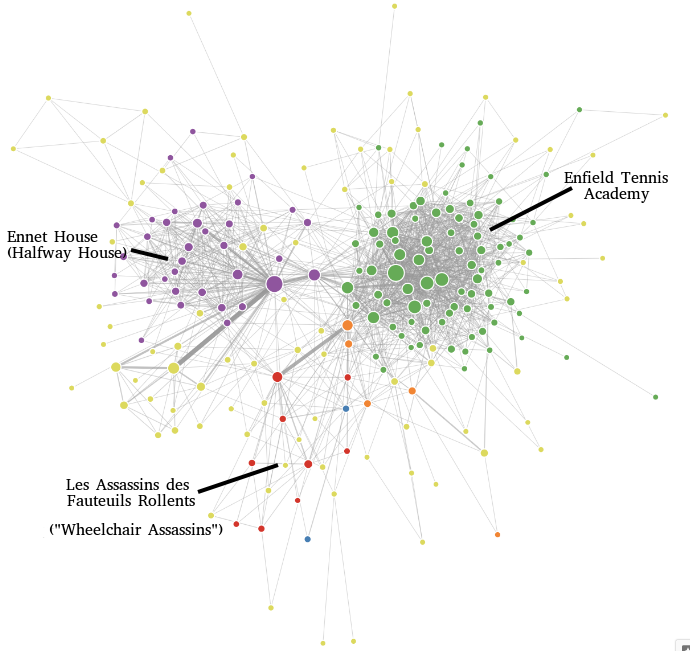
\includegraphics[width=1.\textwidth]{images/labeled_community_with_labels.png}
        \caption{Hand-labeled communities.}
    \end{subfigure}
    \begin{subfigure}{0.4\textwidth}
        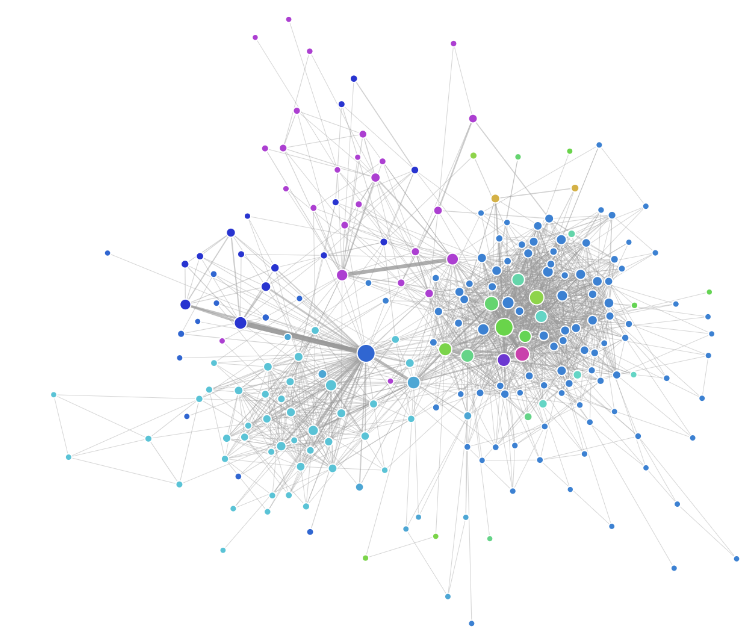
\includegraphics[width=1.\textwidth]{images/greedy_community.png}
        \caption{Communities detected by greedy modularity maximization.}
    \end{subfigure}
    \caption{The agglomerative greedy approach to modularity maximization recovered the hand-labeled communities.}
    \label{fig:modularity}
\end{figure}

The labeled communities and detected communities are visible in Figure \ref{fig:modularity}.

\subsection{Assortativity}
Since the network has clear community structure, we can begin to ask if characters in the network are associated with other characters according to certain attribute similarities. We examine gender assortativity and degree assortativity.

\subsubsection{Degree Assortativity}
We see an unweighted degree assortative mixing coefficient of -0.0945.
Degree assortative networks typically reflect core-periphery structures, where a dense core of highly-connected nodes is surrounded by successively less-dense periphery nodes. Degree disassortative networks, on the other hand, are more stars with high-degree nodes connected to low-degree. 

According to Newman in {\em Networks}, social networks are unusual in that they typically have a positive degree assortativity \cite{NewmanBook}. 
Therefore it is strange for us to see disassortative mixing by degree in \infinitejest, possibly indicating more of a star-like structure or fewer community structures than real-world social networks.

\subsubsection{Gender Assortativity}
To examine gender assortativity, we labeled all of the characters with a gender attribute where the gender was clear from the text. Of 229 nodes, we did not assign a label to 27 of them. We found the assortativity to be 0.0858, indicating positive assortative mixing by gender: genders of the same type are more likely to co-occur in this text. 

This is somewhat expected from the narrative structure, because Hal is a teenager and all of the men board together in the Tennis Academy.

\subsection{Centralities}

\begin{table}[]
\begin{tabular}{@{}lllll@{}}
\toprule
 & \multicolumn{4}{c}{\textbf{Centralities}} \\ \midrule
 & \multicolumn{2}{l}{\textbf{Degree}}  & \multicolumn{2}{l}{\textbf{Betweenness}} \\ \midrule
\textbf{1} & Hal Incandenza   & 0.382 & Donald Gately   & 0.259 \\ \midrule
\textbf{2} & Donald Gately    & 0.311 & Hal Incandenza  & 0.140 \\ \midrule
\textbf{3} & Avril Incandenza & 0.294 & Joelle Van Dyne & 0.079 \\ \midrule
\textbf{4} & Aubrey DeLint    & 0.268 & Charles Tavis   & 0.065 \\ \midrule
\textbf{5} & Gerhardt Schtitt & 0.250 & Remy Marathe    & 0.056 \\ \midrule
\textbf{6} & Michael Pemulis  & 0.246 & John Wayne       & 0.051 \\ \midrule
\textbf{7} & Charles Tavis    & 0.232 & Gerhardt Schtitt & 0.049 \\ \midrule
\textbf{8} & James Incandenza & 0.215 & Michael Pemulis  & 0.048 \\ \toprule
\end{tabular}
    \caption{Top degree and betweenness centralities.}
    \label{tab:centralities}

\end{table}

Centralities answer the question of the most ``important'' vertices in the graph. Since we are analyzing \infinitejest, the question becomes which are the most important characters in the book. There are of course many contexts we could analyze importance from. To most closely align with the concept of main characters in books, we suspect simple degree centrality gives the best answer, since main characters tend to be mentioned more. 

However one could make an argument that in a novel with lots of moving parts, the most important characters might be the ones which connect disparate parts of the plot together and help drive it forward. In that respect, betweenness centrality shines. In \infinitejest, Don and Joelle are the only characters with significant interactions in both communities. Don also has interactions with the Wheelchair Assassins.

The top eight characters under degree and betweenness centralities can be found in Table \ref{tab:centralities}.



\subsection{Gender}

\infinitejest has received significant criticism for its treatment of women.\cite{hayes-brady_2017} We found $144$ male entities, $58$ female entities, and $27$ entities of indeterminate gender or whose gender was unknown; there are nearly two-and-a-half times as many men as women.

\subsubsection{Average Degree}
Figure~\ref{average-node-degree-by-gender} shows the difference in average degree by gender. Average unweighted degree can be seen as a rough approximation for the expected connectedness of a character. Average weighted degree can be seen as a rough approximation of the expected strength of a character's relationships. There is a difference between the average unweighted degrees of men and women, but it far less striking than the difference between their average weighted degrees. 

\begin{figure}[ht!]
    \centering
    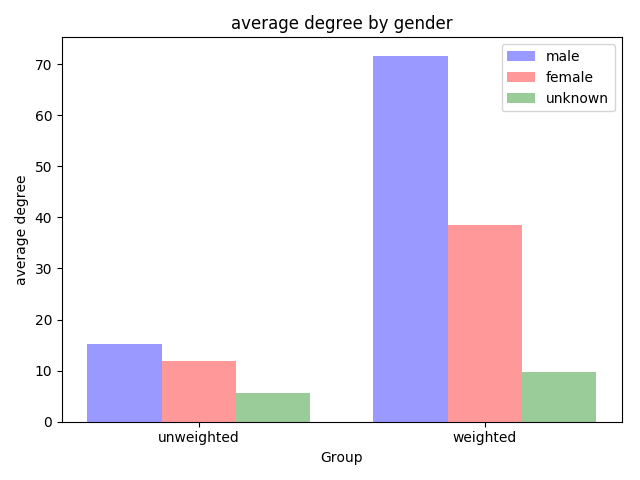
\includegraphics[width=.4 \textwidth]{images/gender_degrees.png}
    \caption{weighted and unweighted average node degree by gender}
    \label{average-node-degree-by-gender}
\end{figure}

\subsubsection{Betweenness}
To explore gender bias in character betweennesses, we ran 100 simulations configuration model using the book's degree sequence, averaging the resulting betweennesses by character. Figure~\ref{difference-in-betweenness} plots a histogram of the differences between the book's betweennesses and our estimates. It shows that, independent of gender, most characters have a significantly lower betweenness in the book than the simulations would lead us to expect, but that several characters in the book have wildly higher betweennesses. It is worth noting that no characters with an indeterminate gender, or whose genders were unknown, had a significantly higher betweenness than expected.

Our findings on the whole indicate that there are several male and female characters who have a priviliged position in the network. Unsurprisingly, these privileged characters are all important: Donald Gately, Joelle van Dyne, Avril Incandenza, and Hal Incandenza are among them. A high betweenness seems like a reasonable consequence of narrative attention.
   
\begin{figure}[ht!]
    \centering
    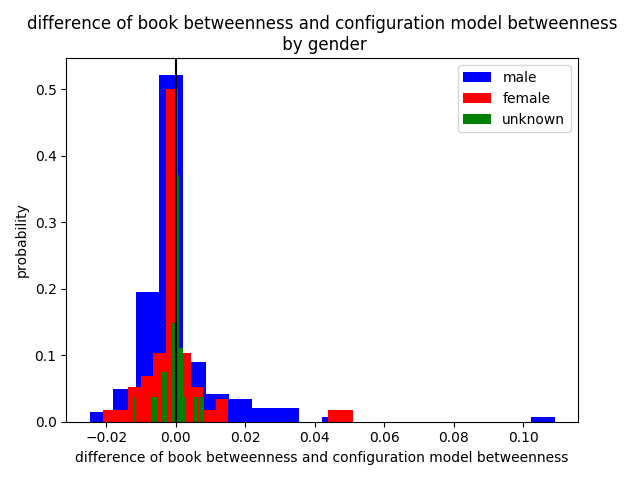
\includegraphics[width=.4 \textwidth]{images/gender_betweenness_by_gender.png}
    \caption{difference in book's betweennesses and those expected under the configuration model, by gender}
    \label{difference-in-betweenness}
\end{figure}

\subsubsection{Degree Sequence}
 

\begin{figure}[ht]
    \centering
    \begin{subfigure}{0.4\textwidth}
        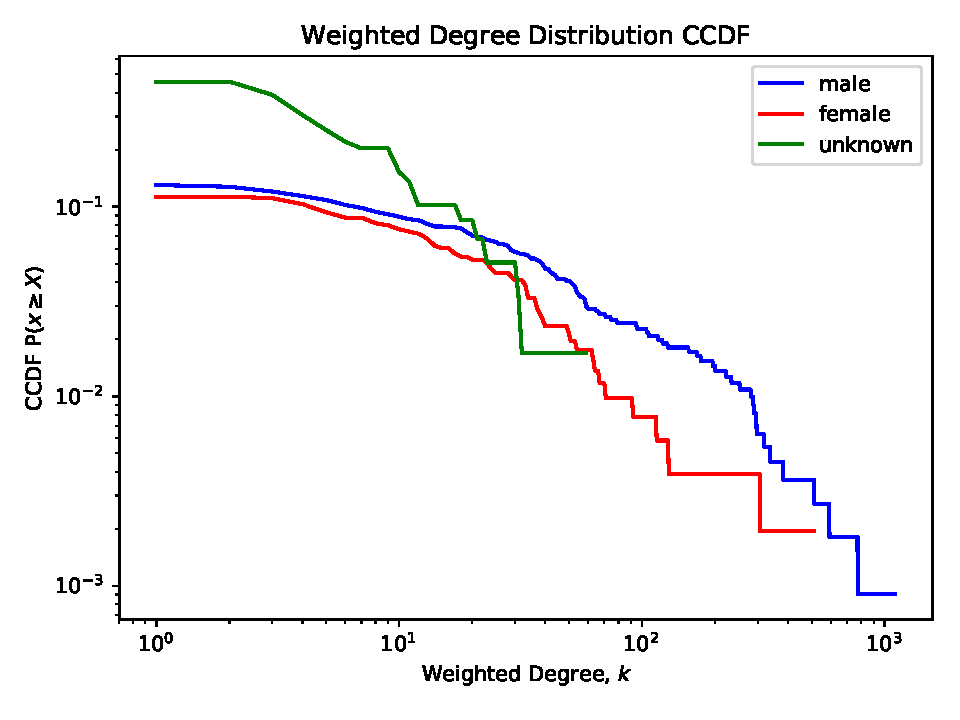
\includegraphics[width=1.\textwidth]{images/degree_distr_ccdf_gender_weighted-Weighted.pdf}
        \caption{Weighted degree distribution by gender}
    \end{subfigure}
    \begin{subfigure}{0.4\textwidth}
        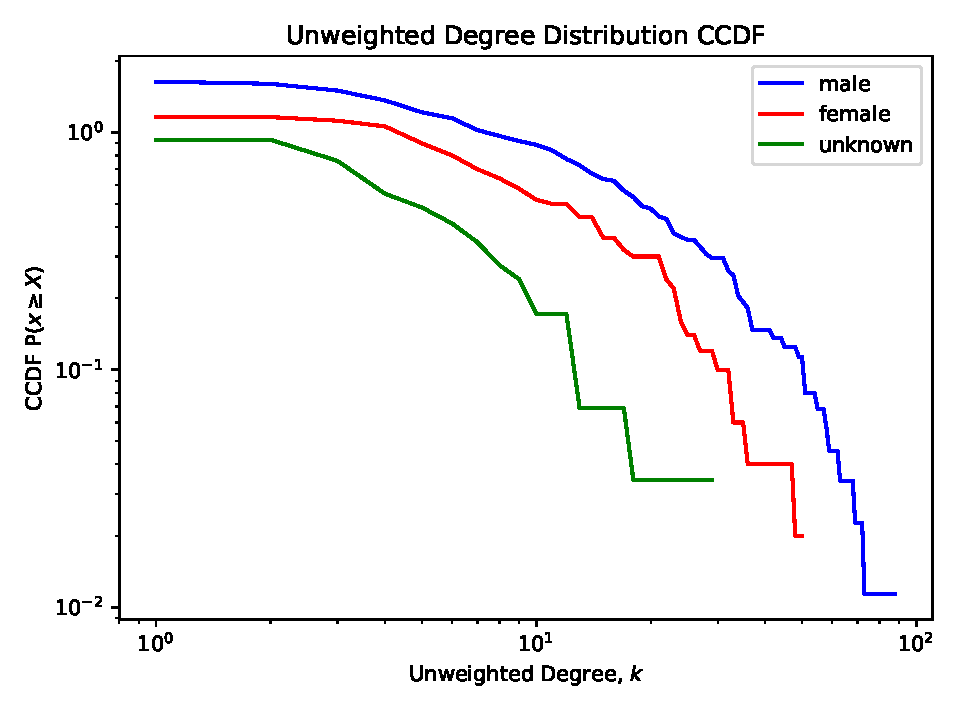
\includegraphics[width=1.\textwidth]{images/degree_distr_ccdf_gender_weighted-Unweighted.pdf}
        \caption{Unweighted degree distribution by gender}
    \end{subfigure}
    \caption{Degree distributions by gender on a log-log scale.}
    \label{fig:degree_distr}
\end{figure}

